\begin{activity} \label{A:7.6.2}  
  Consider the logistic equation
  $$ \frac{dP}{dt} = kP(N-P) $$
  with the graph of $\frac{dP}{dt}$ vs.~$P$ shown below.
  \begin{center}
    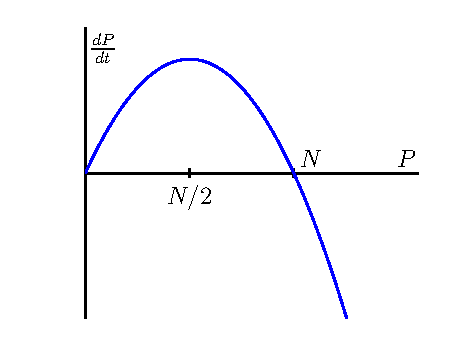
\includegraphics{figures/7_6_activity_2.eps}
  \end{center}
\ba
\item At what value of $P$ is the rate of change greatest?

\item Consider the model for the earth's population that we created.
  At what value of $P$ is the rate of change greatest?  How does that
  compare to the population in recent years?

\item According to the model we developed, what will the population be
  in the year $2100$?

\item According to the model we developed, when will the population
  reach $9$ billion?

\item Now consider the general solution to the general logistic initial value problem that
  we found, given by
  $$
  P(t) = \frac{N}{\left(\frac{N-P_0}{P_0}\right)e^{-kNt} + 1}.
  $$
  Verify algebraically that $P(0) = P_0$ and that $\lim_{t\to\infty} P(t) = N$.

\ea
\end{activity}
\begin{smallhint}
\ba
	\item Small hints for each of the prompts above.
\ea
\end{smallhint}
\begin{bighint}
\ba
	\item Big hints for each of the prompts above.
\ea
\end{bighint}
\begin{activitySolution}
\ba
	\item Solutions for each of the prompts above.
\ea
\end{activitySolution}
\aftera